%!TEX root = ../rapport.tex
%!TEX encoding = UTF-8 Unicode

% Chapitres "Introduction"

% modifié par Francis Valois, Université Laval
% 31/01/2011 - version 1.0 - Création du document


\label{s:experimentation}
\chapter{Laboratoire 2}
\section{Projet 1}

L'objectif fondamental de ce laboratoire est de réaliser un programme informatique qui aura pour fonction de calculer numériquement les paramètres d'une ligne microruban. Le premier paramètre à trouver est l'impédance caractéristique de ligne : $\bar{Z_0}$. Le second paramètre à déterminer est la vitesse de propagation $v_p$.

\paragraph{}
On cherche à identifier les concepts de base théoriques utiles à ce laboratoire, soit :

\begin{itemize}
\item la version numérique de l'intégrale de Gauss nécessaire pour obtenir les capacitances $\mathcal{C}$ et $\mathcal{C}_0$;
\item l'obtention de $Z_0$ et $v_p$ en mode quasi-TEM.
\end{itemize}

\subsection{Passage de l'analytique au numérique}
Les équations de Maxwell permettent, à partir d'une distribution de potentiel qui possède une géométrie simple et d'une distribution d'un champ électrique associé ($\bar{E}$), de déterminer la charge emmagasinée dans une distribution donnée. On observe que le champ électrique d'une distribution est lié au potentiel électrique de la manière suivante :

\begin{equation}
	\vec{E}(x,y) = - \Delta V(x,y)
\end{equation}

Aussi, on sait que la charge électrique dans un milieu donné s'exprime comme : 

\begin{equation}
	Q = \oint_S \! \epsilon \vec{E} \, \mathrm{d}S
\end{equation}

En combiant les deux expression précédentes, on obtient : 

\begin{equation}
	\label{eq:Q}
	Q = \oint_S \! -\epsilon \Delta V(x,y) \, \mathrm{d}S
\end{equation}

On note tout de suite que tout dépendant de l'orientation des surgaces respectives, l'intégrale deviendra rapidement infaisible à la main, dumoins dans un laps de temps court. Il va de soit qu'il est possible d'exprimer ce calcul sous la forme de somme discrète (ce qui est en fait une intégrale) et qu'en minimisant les distances successives d'évaluation, on obtiendra une évaluation de plus en plus précise. On peut penser à une somme de Riemann classique, dans laquelle si on diminuait le pas entre chaque rectangle, on convergerait vers la définition de l'intégrale. En reportant ce résultat dans le cas étudié, on obtient une version discrète de l'équation \ref{eq:Q}.

\subsection{Détermination de \textit{C}}
Afin de déterminer la capacité $\mathcal{C}$, on utilise le résultat qui nous donne une version discrète de la charge électrique de Q en chaque point. Sachant la charge électrique, il suffit de diviser par le potentiel en chaque point. Par la suite, on divise par le pas utilisé (il est intéressant de remarquer que dans le cas où il est uniforme et égal à 1, soit dans notre cas, cette étape n'affecte pas le résultat) et on obtient la capacité totale dans la géométrie étudiée.

\subsection{Détermination de $\epsilon_{r_{interface}}$}
Pour les points placés aux interfaces entre les deux diélectriques, on peut approximer la permittivité à l'interface ($\epsilon_{r_{interface}}$) par : 

\begin{equation}
	\epsilon_{r_{interface}} \approx \frac{ (\epsilon_{r1}+\epsilon_{r2})}{2}
\end{equation}

\subsection{Dètermination de la permittivité effective $\epsilon_{r_{eff}}$}
Dans ce laboratoire, la détermination de la capacité $C$ est faite dans la section précédente. Ce faisant, on peut utiliser le résultat précédent et la relation suivante:

\begin{equation}
	\epsilon_{r_{eff}} = \frac{\mathcal{C}}{\mathcal{C}_0}
\end{equation}

Connaissant $\mathcal{C}$ et $\mathcal{C}_0$, trouver $\epsilon_{r_{eff}}$ devient trivial.

\subsection{Détermination de $Z_0$ et de $v_p$}
Comme on connait $\mathcal{C}$ et $\mathcal{C}_0$ des étapes précédentes, il suffit d'appliquer les relations suivantes pour trouver les deux paramètres demandés : 

\begin{equation}
	V_p \approx c\sqrt{\frac{\mathcal{C}_0}{\mathcal{C}}}
\end{equation}

\begin{equation}
	Z_0 \approx \frac{1}{c\sqrt{\mathcal{C}_0\mathcal{C}}}
\end{equation}


\newpage
\section{Projet 2}
Il est important de noter que dans un soucis de lisibilité, le code Matlab de la fonction MDF n'est pas reporté dans le présent rapport. Celui-ci est toutefois disponible dans le rapport du laboratoire 1.

\subsection{Algorithme}
\subsubsection{Fonction IGauss}

\begin{lstlisting}
function C = IGauss(V, er1, er2, d, w)
    %Largeur et hauteur de la matrice avec correction
    [n,m] = size(V);
    n = n-1;
    m = m-1;
    
    %Milieu du systeme pour le calcul de Vab
    if mod(m+1,2) == 0
        halfM = (m+1)/2;
    else
        halfM = floor((m+1)/2);
    end 
    
    %Definition des constantes
    e0 = 8.854*(10^(-12));
    Vab = V(n+1-d,halfM);
    
    %Remplissage des permitivites pour simplifier les boucles
    permitivityMatrix = zeros(n+1, m+1);
    if d == 0; 
        permitivityMatrix(2:n, 2:m) = er2;
    else
        permitivityMatrix(2:n-d, 2:m) = er2;
        permitivityMatrix(n+1-d, 2:m) = (er1+er2)/2;
        permitivityMatrix(n+2-d:n, 2:m) = er1;
    end
    
    %Calcul du potentiel pour le pourtour du systeme
    tourPotential = 0;

    %Nord et Sud
    for i=2:m   
        tourPotential = tourPotential + permitivityMatrix(n,i)*V(n,i);
        tourPotential = tourPotential + permitivityMatrix(2,i)*V(2,i);
    end
    
    %Est et Ouest
    for i=2:n
        tourPotential = tourPotential + permitivityMatrix(i,2)*V(i,2);
        tourPotential = tourPotential + permitivityMatrix(i,m)*V(i,m);
    end
    
    %Calcul de la capacite
    C = e0/Vab*tourPotential; 
end
\end{lstlisting}
\subsubsection{Fonction MicroPar}
\begin{lstlisting}
	function [Z_o, v_p] = MicroPar(m, n , er1, er2, d, w, tol)
	    %Declaration des constantes
	    c = 3*(10^8);
    
	    %Creation des deux matrices de potentiel. La premiere avec une
	    %permitivite dans le vide et l'autre avec les permitivites originales
	    V_vide = mdf(m,n,1,1,d,w,tol);
	    Vp_orig = mdf(m,n,er1,er2,d,w,tol);
    
	    %Calcul des deux differentes capacites
	    C0 = IGauss(V_vide,1,1,d,w);
	    C = IGauss(Vp_orig,er1,er2,d,w);
    
    
	    %Calcul des valeurs demandees selon les equation 1.6 et 1.7 dans le
	    %rapport
	    Z_o = 1/(c*sqrt(C0*C));
	    v_p = c*sqrt(C0/C);
	end
\end{lstlisting}

\subsection{Guide d'utilisation}

\textit{Les fichiers nommés mdf.m, IGauss.m et MicroPar.m sont disponibles dans le répertoire remis sur pixel.}
\begin{enumerate}
\item Copier les fichiers dans un répertoire connu du logiciel Matlab;
\item Dans l'interpréteur, fixer les paramètres d'appel de la fonction selon la même nomenclature qu'utilisée dans l'énoncé de laboratoire. Pour se faire, utiliser une syntaxe du genre: m=10; etc. 
\begin{itemize}
\item \textit{Exemple:} [Z0, vp] = MicroPar(10,10, 1.10,4,3,$1*10^{(-9)}$);
\end{itemize}
\item Interpréter la ligne (appuyer sur entrer);
\item Le "workspace" de Matlab devrait contenir les deux réponses voulues.
\end{enumerate}

\section{Projet 3: Reproduction des exemples}
Sachant que dans le précédent rapport, les deux matrices obtenues étaient en tout point semblables à celles fournies, il ne sert a rien de réeffectuer la comparaison.
\subsection{Exemple 7.5}

La matrice obtenu par la fonction mdf avec un seuil de tolérence de $10^{-9}$ par notre programme est la suivante :
\[V_0  = \left(\begin{array}{ccccccc}
0 & 0 			& 0 			& 0 			& 0 			& 0 			& 0 \\
0 & 0.07043930 	& 0.12599118 	& 0.14570741	& 0.12599118	& 0.07043930 	& 0 \\
0 & 0.15576603 	& 0.28781803 	& 0.33084727 	& 0.28781803 	& 0.15576603 	& 0 \\
0 & 0.26480681 	& 0.53866761 	& 0.60204562  	& 0.53866761 	& 0.26480681 	& 0 \\
0 & 0.36479358 	& 1				& 1				& 1			 	& 0.36479358 	& 0 \\
0 & 0.19436750 	& 0.41267643 	& 0.45633821	& 0.41267643 	& 0.19436750 	& 0 \\
0 & 0 			& 0 			& 0 			& 0 			& 0 			& 0 
\end{array} \right)\]

En utilisant cette matrice dans la fonction IGauss ainsi que les paramètres suivants : 

\begin{itemize}
\item $\epsilon_{r1}$ = $\epsilon_{r2}$ = 1;
\item $\omega$ = 2;
\item d = 2.
\end{itemize}
nous donnes la capacité suivante :

\begin{equation}
	C_0 \approx 38.1549044906185 [pF/m]
\end{equation}

Cette valeur est très proche de la valeur fournie qui est la suivante :

\begin{equation}
	C_{0_{prof}} \approx 38.15571464671 [pF/m]
\end{equation}

La différence entre les deux valeurs est de moins de 0.002\% ce qui semble est un taux d'erreur très acceptable.
\subsection{Exemple 7.6}
La matrice obtenu avec un seuil de tolérence de $10^{-9}$ par notre programme est la suivante : 

\[V  = \left(\begin{array}{ccccccc}
0 & 0 			& 0 			& 0 			& 0 			& 0 			& 0 \\
0 & 0.06983505 	& 0.12534299 	& 0.14509465	& 0.12534299	& 0.06983505 	& 0 \\
0 & 0.15399721 	& 0.28644227 	& 0.32969262 	& 0.28644227 	& 0.15399721 	& 0 \\
0 & 0.25971150 	& 0.53673627 	& 0.60079129  	& 0.53673627 	& 0.25971150 	& 0 \\
0 & 0.34811255 	& 1				& 1				& 1			 	& 0.34811255 	& 0 \\
0 & 0.18987646 	& 0.41139327 	& 0.45569664	& 0.41139327 	& 0.18987646 	& 0 \\
0 & 0 			& 0 			& 0 			& 0 			& 0 			& 0 \\
\end{array} \right)\]
\newline
\newline
En utilisant cette matrice dans la fonction IGauss ainsi que les paramètres suivants : 

\begin{itemize}
\item $\epsilon_{r1}$ = 10
\item $\epsilon_{r2}$ = 1;
\item $\omega$ = 2;
\item d = 2.
\end{itemize}
nous donnes la capacité suivante :

\begin{equation}
	C_0 \approx 227.651093653445[pF/m]
\end{equation}

Cette valeur est très proche de la valeur fournie qui est la suivante :

\begin{equation}
	C_{0_{prof}} \approx 227.6559274467 [pF/m]
\end{equation}

Encore une fois, la différence entre les deux valeurs est de moins de 0.002\% ce qui tend a prouver que la fonction fait bien ce qui lui est demandé.

\section{Projet 4:  selon la géométrie et les diélectriques}

Les figures obtenues pour les exemples demandés sont présentées à la figure \ref{fig_marde}.Les figures obtenues pour l'exemple supplémentaire demandé sont présentées à la figure \ref{mangedlamarde}.

\begin{figure}[htb]
\begin{center}
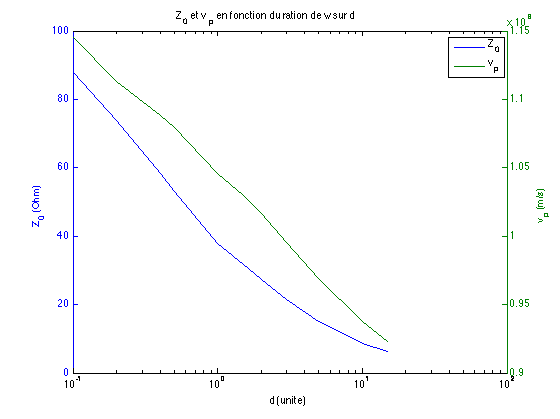
\includegraphics[scale=0.7]{photo1.png}
\label{fig_marde}
\caption{Figures représentant les propriétés intrinsèques de la géométrie du microruban ($Z_0 (\frac{w}{d})$ et $v_p(\frac{w}{d})$) pour les caractéristiques données dans l'énoncé du projet IV}
\end{center}
\end{figure}
\begin{figure}[htb]
\begin{center}
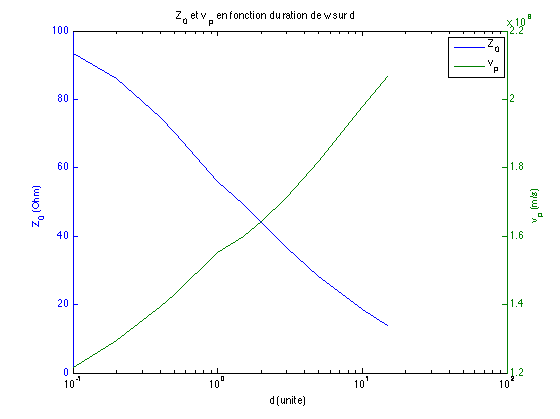
\includegraphics[scale=0.7]{photo2.png}
\caption{Figures représentant les propriétés intrinsèques de la géométrie du microruban ($Z_0 (\frac{w}{d})$ et $v_p(\frac{w}{d})$) pour les caractéristiques données dans l'énoncé du projet IV, mais avec les permittivités $\epsilon_{r1}$ et $\epsilon_{r2}$ inversées}
\end{center}
\label{mangedlamarde}
\end{figure}

\paragraph{}On remarque que dans le second exemple, la courbe de l'impédance intrinsèque ($Z_0$) est similaire à celle du premier, mais que la courbe de vitesse de propagation ($v_p$) a sa croissance inversée. Pour s'en convaincre on procède à un example limite où les deux permittivités sont égales. Cet exemple additionnel est présenté à la figure \ref{mangemoilcul}

\begin{figure}[htb]
\begin{center}
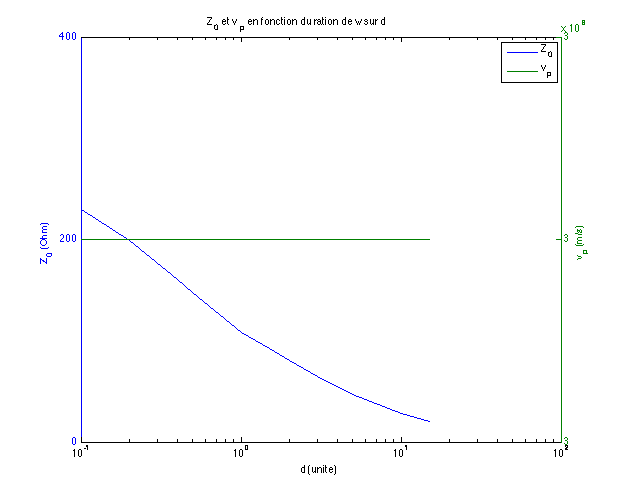
\includegraphics[scale=0.7]{photo3.png}
\label{mangemoilcul}
\caption{Figures représentant les propriétés intrinsèques de la géométrie du microruban ($Z_0 (\frac{w}{d})$ et $v_p(\frac{w}{d})$) pour les caractéristiques données dans l'énoncé du projet IV, mais avec les permittivités $\epsilon_{r1}$ et $\epsilon_{r2}$ égales à 1}
\end{center}
\end{figure}

\paragraph{}On note alors que dans cet exemple limite, la vitesse de propagation $v_p$ est constante et que que $Z_0$ possède la même forme de courbe que les exemples précédents. 


